%
% $Id: ch01_overview
%
%   *******************************************************************
%   * SEE THE MAIN FILE "AllegThesis.tex" FOR MORE INFORMATION.       *
%   *******************************************************************

\chapter{Introduction}\label{ch:intro} % we can refer to chapter by the label

%   ************************************************************************
%   * In LaTeX, new paragraphs are begun by simply leaving a blank line in *
%   * the LaTeX file.                                                      *
%   *                                                                      *
%   * The \\ characters should NEVER be used to end a paragraph.           *
%   * They are used only for inserting line breaks in certain situations.  *
%   *                                                                      *
%   * "Widows" (ending paragraph lines at the top of a new page) and       *
%   * "orphans" (opening paragraph lines at the bottom of a page) should   *
%   * be eliminated; this sometimes requires re-writing some of the        *
%   * text to change the line lengths.                                     *
%   ************************************************************************


%The purpose of this sample thesis is to show various \LaTeX\ formatting
%commands. Information about content should be obtained through consultation
%with the thesis readers and examination of past senior theses.
%There are no fixed rules governing the number of chapters or their titles---old 
%senior theses and discussions with the thesis readers are the best resources
%for making such decisions.

%Usually, a chapter begins with a paragraph or two that serves as a
%sort of mini-introduction to the chapter. This is followed
%by numbered sections created with ``\verb$\section{...}$'', 
%``\verb$\subsection{...}$'', etc.




\section{Motivation} \label{sec:motivation}
%The first paragraph in each section is not indented---that is a standard style
%that is enforced by the \LaTeX\ program. It should never be necessary to
%insert commands to force paragraph indentation.

When programmers write code in Java programming language, there is a high chance that some of the programs do not run as expected. There are many options to fix this issue. One approach is to look back into the source code and read it line-by-line and try to find out what the issue is. This approach is time consuming and tiresome and may not always work. An alternative approach is to use a tool such as FindBugs, PMD, or Checkstyle to help finding the issue.
\newpage
\begin{figure}[htbp]
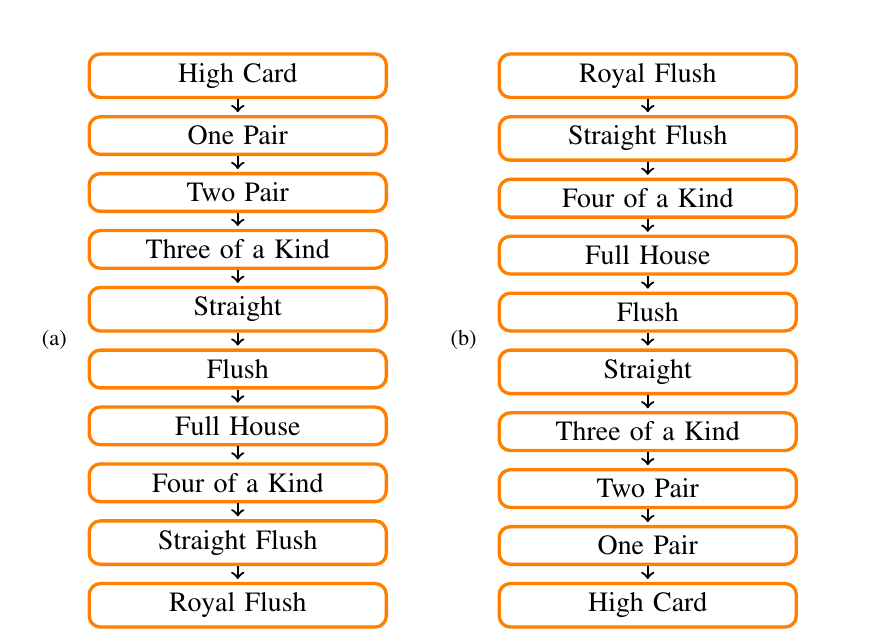
\includegraphics[scale=0.4]{motivationImproved.png}
\caption{The Figure shows the representation of poker hands - (a) starts with the lowest hand (b) starts with the highest hand. The highest hand is the winner of the game, and therefore the program code should use the representation (b) to decide the winner.}
\label{fig:pr}
\end{figure}


For example, let us say we are writing a program in Java that will decide the winner of a poker game. Figure 1.1 shows the different poker hands that a player can have. Figure 1.1 (a) shows the sequence of hands starting with the lowest hand `high card' and ending with the highest hand `royal flush', where figure 1.1 (b) starts with the highest hand `royal flush' and ends with the lowest hand `high card'.
The program is written so it looks at poker hands starting at the beginning of the representation and continues to go through the poker hands in the representation until a match between the poker hand and the representation is found. If there is a match the program will select the hand as the highest hand.
Using the representation in Figure 1.1 (a) the program will start with the `high card'. A poker hand always has a highest card so it will stop here and select the highest card as the poker hand. This is not correct because there could also be `one pair', `two pair', `three of a kind' or any of the other hands listed in the representation. Using this representation will not necessarily find the highest poker hand.      
Using the representation in Figure 1.1 (b) the program will go through the representation starting with the highest hand, and select the first match, which will give the highest hand and this is correct.

Figure 1.1: The Figure shows the representation of poker hands - (a) starts with the lowest hand and (b) starts with the highest hand. The highest hand is the winner of the game, and therefore the program code should use the representation (b) to decide the winner.  



%For example, let us say we are writing a program in Java to decide the winner of the poker game. Figure \ref{fig:pr} shows the different poker hands that a player can have. Figure \ref{fig:pr} (a) shows the sequence of hands starting with the lowest hand, `high card' and ending with the highest hand, `royal flush' where Figure \ref{fig:pr} (b) starts with the highest hand, `royal flush' and ends with the lowest hand, `high card'. The representation in Figure \ref{fig:pr} (a) would not be correct to use in the program because the program would look for a lower hand before it looks for a higher hand and therefore not select the highest possible hand. To fix this issue, the program should use the representation shown in Figure \ref{fig:pr} (b) to evaluate the winning hand of the poker game. The tools FindBugs, PMD, and Checkstyle will be evaluated to find out if they could suggest that the bug is in the sequence of the poker hand representation.   

%shows the correct representation on how to follow a game of poker. Figure \ref{fig:pr} (a) would be a wrong because a program is looking for a hand that contains a pair before they look for a hand that could possibly have two pairs inside it. Therefore this design will not select the highest possible combination. To fix this, Figure \ref{fig:pr} (b) would be the correct representation of how a game of poker should be played. The tools of FindBugs, PMD and Checkstyle will be evaluated to see if they ciouyld suggest the big is in the sequence of the poker hand representation.

%The thesis should avoid the use of second-person pronouns such as ``you''
%and ``your,'' as well as the use of imperative statements (implied
%second-person) such as ``Look
%at \ldots'' or ``Consider the following example \ldots''. 
%First person (``I,'' ``my,'' etc.) is sometimes acceptable, 
%but should be used sparingly. (This is an appropriate topic 
%or discussion with the first reader of the project.) Contractions (``don't'',
%`can't'', etc.) are considered informal and should be avoided. Common
%abbreviations such as ``math'' for ``mathematics'' or ``comp'' for 
%``senior comprehensive project''  are also informal and not appropriate
%in the final thesis.

%Figures illustrating complex or hard-to-describe concepts are essential.
%All figures should be fully explained in the text. For example,
%Figure \ref{latexprocess} shows the first step in processing a senior thesis.
%The user files consist of the main file, {\tt AllegThesis.tex}, and zero or
%ore additional files ({\tt ch01.tex}, {\tt ch02.tex} in the figure). Not shown
%n the figure are image files, the bibliography, and other included
%components (the ``\ldots etc.\ldots'' on the left side of the figure). 
%Typing the command {\tt pdflatex} with the main file name
%produces a number of additional files, including an {\tt .aux} file (with
%information such a label references and citations),
%a table of contents, or {\tt .toc}, file, a printable {\tt .pdf} file, and
%a number of others, depending on the document.

%   *******************************************************************
%   * FIGURES ARE PLACED ACCORDING TO A SET OF CONSTRAINTS THAT CAN   *
%   * BE MANIPULATED TO SOME DEGREE.                                  *
%   * A SEARCH FOR "controlling latex floats" TURNS UP A NUMBER OF    *
%   * SITES THAT HAVE USEFUL INFORMATION, FOR EXAMPLE:                *
%   *                                                                 *
%   * http://mintaka.sdsu.edu/GF/bibliog/latex/floats.html            *
%   * http://goo.gl/aC8E8Q                                            *
%   * http://robjhyndman.com/hyndsight/latex-floats/                  *
%   *******************************************************************

%\begin{figure}[htbp]
%\centering
%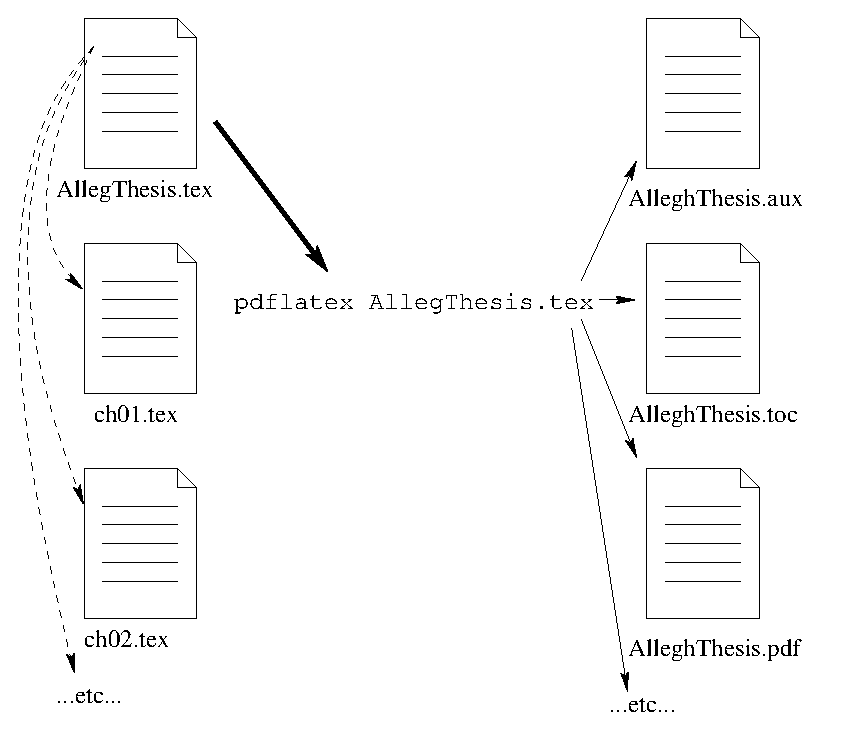
\includegraphics[width=3.5in]{latexprocess}
%\caption{The first step in creating a thesis document}
%\label{latexprocess}
%\end{figure}

\section{Current State of the Art}\label{sec:stateofart}
%There are multiple
%ways to create {\it italicized}, {\bf bold-face}, {\tt fixed-width}, and
%{\sf sans-serif} fonts, as well as combinations, e.g., \textit{\textbf{
%bold italic}} or \textit{\textsf{italic sans-serif}}. The \LaTeX\ source
%file for this chapter shows some of the ways to achieve these effects.
%It is customary to use fixed-width font for program constructs, e.g.,
%`In the Java code accompanying the figure, {\tt n} stands for the 
%umber of generations to be simulated by the {\tt evolvePopulation()} method.'' 
%Variables in mathematical equations are normally rendered in 
%talics, e.g., ``In the performance equation, {\it cpuTime} is 
%the average time over fifty runs of the program.''

%It is the privilege of the thesis author (in consultation with the
%project super(a) shows the wrong representation and (b) shows the correct representation to follow when playing a game of pokervisor and other readers) to decide on the best way to 
%organize the sections and chapters in the way that makes the most sense.
%If the introduction begins with a motivating
%anecdote, perhaps this is best followed by defining a few terms or mentioning
%some major results that the reader should be aware of right from the 
%beginning. But 
%It is important to get as quickly as possible to 
%a concise statement of the {\it thesis}---the main question 
%addressed by the project. This might merit a separate
%ection of the chapter.

At present, the process of locating logic based bugs is mostly manual. However, there are tools to assist in finding logic based bugs. Many of these tools have been developed using techniques such as syntactic pattern matching, data flow analysis, type systems, model checking, and theorem proving \cite{bugFindingTools}.


\section{Definitions}\label{sec:definitions}
 logic based bug is defined as a bug in a program that causes it to operate incorrectly. The program will not terminate abnormally or crash. This is considered to be fault of commission. An example of a logic based bug is comparing String objects with the == operator compared to the .equals() method. When it comes to objects, when using the == operator, it is testing for references equality. This means that it is checking if the two are the same object. The .equals() method tests for value equality. This means that it is testing if the two objects are logically ``equal". 
 
 
 %An example of a logic based bug when you have a program that is supposed to calculate velocity squared. Velocity squared should equal $2 * (kinetic / mass).$ But instead, your program is calculating Velocity squared to be $3 * (kinetic / mass).$ Due to the fact that the program does not follow the law of physics, this is considered to be a logic based bug. 
 
Source code analysis is defined as: ``Source code analysis is the process of extracting information about a program from its source code or artifacts generated from the source code using automatic tools" \cite{Binkley}. The idea of source code analysis is imperative in order to figure out how programs works. Source code analysis is also used to locate bugs in programs.
  
 Static program analysis of software is defined as analysis that is completed without actually executing programs and is usually performed as part of a Code Review. The analysis attempts to highlight possible errors within the source code. The three tools analyzed in this paper FindBugs, PMD, and Checkstyle are examples of static program analysis. These tools intend to identify errors in Java code without running the program. 
 %The tools are grouped into four types. The first group is code analysis where statements are highlighted if the syntax is wrong. logic based bugs
 %This group generates a graph from the components submitted as input. The third group is called data analyzers and reviews the data structures to identify improper linkage among components. The fourth and last group is called a sequence checker and checks the sequences of events. Events that might be coded in an incorrect sequence are highlighted.

Dynamic Program Analysis is defined as the analysis of computer software that is performed by executing programs on a real or virtual processor. Tools using Dynamic Program Analysis are also known as program monitors because they watch and report the program's behavior. 

Fault of omission is when some key aspect of the code is missing. For example, when a variable is not initialized.

Fault of commission is when there are one or more 
incorrect assignments in a program. For example, when a variable is initialized to the wrong value.

Compiler bug is defined as a bug that is detected by the compiler when compiling the source code and it prevents it from being executable. An example of a compiler bug is writing a line of source code without a semi colon (;) at the end of the statement.

 Run-time bug is defined as a bug that occurs during the execution of a program. In contrast to logic based bugs, a run-time bug will terminate or crash the program. 

 False Positive is defined as a condition that is incorrectly reported as an error. For example the tools FindBugs, PMD, or Checkstyle could report a false positive if they scan through source code and highlight lines in the code that actually do not contain any bug.  
 
 False Negative is defined as a condition where a test result improperly indicates no presence of an error. For example tools FindBugs, PMD, or Checkstyle could report a false negative if they scan through source code and fail to highlight lines of the code that actually hold bugs. 
 
 Cyclomatic Complexity is defined as a measurement used to indicate the complexity of a program. This  metric calculates the number of linearly independent paths through a program's source code. The tool PMD is able to measure the complexity of a program by calculating the number of linearly independent paths in a program's source code.

 Inefficient Code is when complex code can be re-written to be simpler. An example of inefficient code in Java is using the String.trim().length() to check if a string is empty. This approach creates a new String object just to check its size. Instead a static function that loops through the string should be used as this would be a much more efficient way to check if a string is empty. 
 
 Bug checker is defined as a static analysis tool used to find code that does not conform to specific properties and which may cause the program to misbehave at runtime \cite{bugFindingTools}. An example of a bug checker is the tool FindBugs.
 
 Style checkers examine code to determine if it contains non-conformance to particular coding style rules \cite{bugFindingTools}. Enforcing style checkers create a consistent style throughout  programs and projects. This makes it easier for developers to understand and maintain code for a particular project. Two examples of style checkers are PMD and Checkstyle.




\section{Goals of the Project}\label{sec:goals}
%This section could also be entitled ``Thesis'' or something similar. 
There are two significant goals for this project. The first goal is to perform the empirical study of the tools and this goal is a prerequisite for the second goal. The second goal is to determine whether new tools should be developed or additional features could be added to one or more of the existing tools. If none of the three tools FindBugs, PMD, and Checkstyle are successful in assisting the programmer in finding logic based bugs then it may be recommended that a new tool should be developed. However, if at least one of the three tools are able to successfully assist in locating the bugs, then the tool may be the future tool used to assist in such a tedious and time-consuming task. 
 
%A formal thesis statement should be a 
%\emph{falsifiable} % COMMENT OUT THINGS THAT YOU MAY LATER WISH TO PUT BACK
%statement about 
%the goal achieved by the project.  For a purely scientific
%project, this is the hypothesis being tested; it should be a
%\emph{falsifiable} statement, i.e., one that can be disproven through
%an appropriate experiment.
%For an applied programming project, it is usually a statement about 
%the feasibility and correctness of the approach used and the advantages it 
%has over other approaches, using suitable metrics.  For a survey or study,
%it is usually a statement regarding the need 
%or usefulness of such a study, its intended audience, and so on.

% COMMENTED OUT NEXT FEW LINES TO SAVE SPACE; MAY PUT THEM BACK LATER
%Following the concise statement of the thesis, some of the details can be
%expanded.  
%It is appropriate to
%refer to some of the results in the introduction (which may 
%mean going back and adding them to the introduction once the
%research is completed). 
%A senior thesis, or any research paper, is not a mystery 
%novel---there is no need to keep the reader in suspense about what
%has been accomplished.

\section{Thesis Outline}\label{sec:outline}
%The introductory chapter usually concludes with a ``road map'' of the upcoming
%chapters, e.g., ``Chapter \ref{ch:relatedwork} reviews a number of past approaches
%to the problem and summarizes their strengths and weaknesses. Chapter 
%\ref{ch:method} outlines the method of approach used to establish the
%results.''

This paper consists of eight chapters which cover topics for my senior project. Chapter 2 will discuss the related research work that is on-going in the field of assisting in locating logic bugs. Chapter 3, 4, and 5 will describe the three tools FindBugs, PMD, and Checkstyle accordingly including their features and functionality. Chapter 6 outlines the methodology I have used for this project including how each participant conducted the study and descriptions of the buggy programs I have developed. In chapter 7 the results of this empirical study are presented and discussed and this is used to form the conclusion. Chapter 8 is the conclusion of my study and it also includes suggestions for further studies.     
